\documentclass[aspectratio=169]{beamer} %[t]:顶端对齐
\usepackage{uni}
%\usetheme{Madrid} %Madrid,蓝色调为主。
%\usecolortheme{beaver} %beaver
%\usefonttheme{professionalfonts}

\date{\today}
\begin{document}

\begin{frame}[fragile]
\frametitle{LaTex在线编辑器}
\underline{\Huge \textbf{\href{https://www.overleaf.com/}{\textcolor{blue}{https://www.overleaf.com/}}}}
\end{frame}

\begin{frame}[fragile]
\frametitle{LaTex文档结构}

\unilstset{TeX}
\begin{lstlisting}
\documentclass{...} % ... 为某文档类
% 导言区
\begin{document}
% 正文内容
\end{document}
% 此后内容会被忽略
\end{lstlisting}

\end{frame}

\begin{frame}[fragile]
\frametitle{LaTex作图模板代码}

\unilstset{TeX}
\begin{lstlisting}
\documentclass [tikz, border=12pt] {standalone}

\begin{document}

\begin{tikzpicture}

%详细作图的指令

\end{tikzpicture}

\end{document}
\end{lstlisting}

\end{frame}

%17.2 函数图象
% 定义一个命令,包含 tikz 图形
\newcommand{\fig}[1][1]{
\begin{figure}
\centering
\begin{tikzpicture}[scale=#1]
  \fontsize{14pt}{16pt}\selectfont % 设置normalsize
  % 绘制坐标轴
  \draw[->, >=stealth] (-3.5,0) -- (3.5,0) node[right] {$x$};
  \draw[->, >=stealth] (0,-3.5) -- (0,3.5) node[above] {$y$};
  
  % 添加x轴刻度
  \foreach \x in {-3,-2,-1,1,2,3}
    \draw (\x,0.1) -- (\x,0) node[below] {$\x$};
  
  % 添加y轴刻度
  \foreach \y in {-3,-2,-1,1,2,3}
    \draw (0.1,\y) -- (0,\y) node[left] {$\y$};

  % 标注原点O
  \node at (0,0) [below right] {$O$};
  
  % 标注象限(使用大写罗马数字)
  \node at (2,2.5) {\textrm{I}};
  \node at (-2,2.5) {\textrm{II}};
  \node at (-2,-2) {\textrm{III}};
  \node at (2,-2) {\textrm{IV}};
  
  % 绘制点P(3,2)及其标签
  \filldraw (3,2) circle (1pt) node[above right] {$P$};
  
  % 绘制虚线投影并标注M、N点
  \draw[dashed] (3,2) -- (3,0);
  \filldraw (3,0) circle (1pt) node[above right] {$M$};
  \draw[dashed] (3,2) -- (0,2);
  \filldraw (0,2) circle (1pt) node[above right] {$N$};
\end{tikzpicture}
\caption{17.2.2}
\end{figure}
}


\begin{frame}{17.2 函数图象(平面直角坐标系)}
\begin{columns}
\column{0.5\textwidth}
\textbf{在数学中,我们可以用一对有序实数来确定平面上点的位置。}\\
\vspace{12pt}
\textbf{\textcolor{orange}{为此,在平面上画两条原点重合、互相垂直且具有相同单位长度的数轴,这就建立了平面直角坐标系(rectangle coordinate system)。}} \\
\vspace{12pt}
\textbf{通常把其中水平的数轴叫做$x$轴或横轴,取向右为正方向;铅直的数轴叫做$y$轴或纵轴,取向上为正方向;两条数轴的交点$O$叫做坐标原点。} \\
\vspace{12pt}
\textbf{为了纪念法国数学家笛卡儿,通常称为笛卡儿直角坐标系。}
\column{0.4\textwidth}
\fig[1.6]

\end{columns}
\end{frame}

\begin{frame}{平面直角坐标系}
\begin{columns}
\column{0.6\textwidth}
%\setlength{\baselineskip}{32pt}  % 设置行间距
\textbf{在平面直角坐标系中,任意一点都可以用一对有序实数来表示。例如,图17.2.2中的点$P$,从点$P$分别向$x$轴和$y$轴作垂线,垂足分别为点$M$和点$N$。}\\
\vspace{12pt}
\textbf{这时,点M在$x$轴上对应的数为3,\textcolor{orange}{称为点P的横坐标(abscissa)。}点$N$在$y$轴上对应的数为2,\textcolor{orange}{称为点$P$的纵坐标(ordinate)。}}\\
\vspace{12pt}
\textbf{依次写出点$P$的横坐标和纵坐标,得到一对有序实数(3, 2),称为点$P$的坐标。这时点$P$可记作$P(3, 2)$。}\\
\vspace{12pt}
\textbf{在平面直角坐标系中,两条坐标轴把平面分成如图17.2.2所示的I、II、III、IV四个区域,\textcolor{orange}{分别称为第一、二、三、四象限。坐标轴上的点不属于任何一个象限。}}

\column{0.3\textwidth}
\fig[1.4]
\end{columns}
\end{frame}

\begin{frame}[fragile]
\frametitle{LaTex作图-画线}

\lstset{
  language=TeX,
  basicstyle=\ttfamily\small,
  backgroundcolor=\color{lightgray},
  keywordstyle=\color{orange},
  commentstyle=\color{red},
  stringstyle=\color{blue},
  frame=single, 
  numbers=left,
  label={lst:sum},
}
\begin{lstlisting}
\documentclass [tikz, border=12pt] {standalone}

\begin{document}
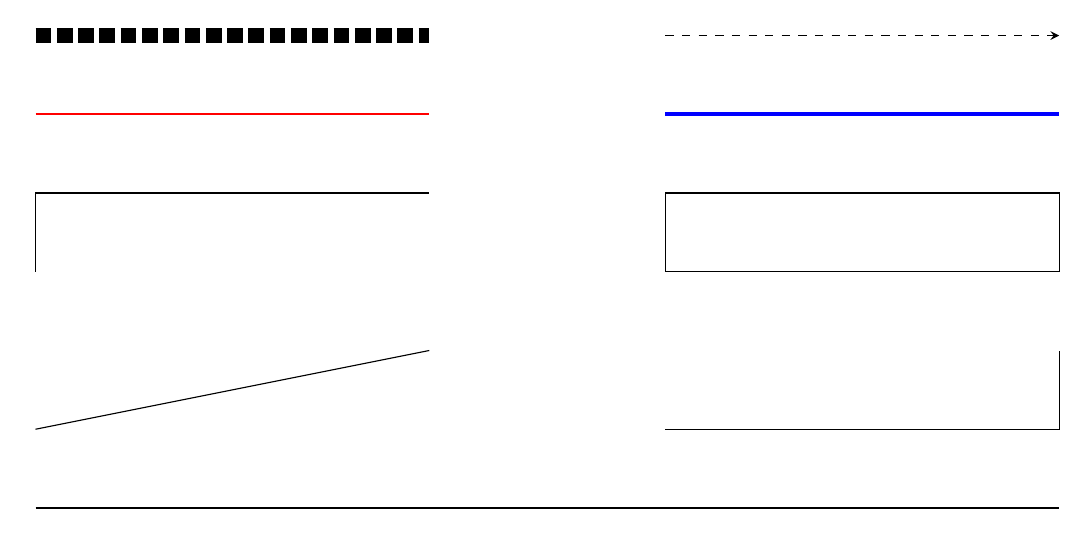
\begin{tikzpicture}

\draw (1,0)  -- (14,0); % 画一条线
\draw (1,1) to (6,2); % 画一条线
\draw (9,1) -| (14,2); % 画一条折线(先水平,后垂直)
\draw (1,3) |- (6,4) ; % 画一条折线(先垂直,后水平)
\draw (9,3) rectangle (14,4); % 画一个矩形
\draw [red,thick] (1,5) -- (6,5); % 红色,粗细:thick
\draw [blue,ultra thick] (9,5) -- (14,5); % 蓝色,ultra thick
\draw [dotted,line width=0.2cm] (1,6) -- (6,6); % 点线,线宽0.2cm
\draw [dashed,->,>=stealth] (9,6) -- (14,6) ; % 虚线,stealth箭头

\end{tikzpicture}
\end{document}
\end{lstlisting}
\end{frame}
\begin{frame}[fragile]
\frametitle{LaTex作图-等边三角形1}

\unilstset{TeX}
\begin{lstlisting}
\documentclass[tikz, border=12pt]{standalone}
\usetikzlibrary{intersections, through}
\begin{document}
\begin{tikzpicture}
    \coordinate (A) at (0, 0); % 定义坐标A
    \coordinate (B) at (5, 0); % 定义坐标B
    \draw[thick, dashed, name path=CA] (A) circle (5); % 绘制圆CA
    \draw[thick, dashed, name path=CB] (B) circle (5); % 绘制圆CB
    \path [name intersections={of=CA and CB, by={P}}]; % 求交点P
    \filldraw[black] (P) circle (1pt); % 给点P画上实心圆
    \draw[thick] (A) -- (P) -- (B) -- cycle; % 绘制等边三角形
    \node[below left] at (A) {A}; % 标注A
    \node[below right] at (B) {B}; % 标注B
    \node[above] at (P) {P}; % 标注P
\end{tikzpicture}
\end{document}
\end{lstlisting}
\end{frame}

\begin{frame}[fragile]
\frametitle{LaTex作图-等边三角形2}

\lstset{
  language=TeX,
  basicstyle=\ttfamily\small,
  backgroundcolor=\color{lightgray},
  keywordstyle=\color{orange},
  commentstyle=\color{red},
  stringstyle=\color{blue},
  frame=single, 
  numbers=left,
  label={lst:sum},
}
\begin{lstlisting}
\documentclass[tikz, border=12pt]{standalone}
\usepackage{tikz}
\usetikzlibrary{intersections}
\begin{document}
\begin{tikzpicture}

\coordinate (A) at (0, 0); % 定义点A
\coordinate (B) at (5, 0); % 定义点B
\draw[name path=A1] (A)+(55:5) arc(55:65:5); % 画圆弧A1,A为圆心,55-65度,半径5
\draw[name path=A2] (B)+(125:5) arc(125:115:5); % 画圆弧A2,B为圆心,125-115度,半径5
\path [name intersections={of=A1 and A2, by=P}]; % 求交点P
\draw[thick] (A) -- (B) -- (P) -- cycle; % 画连接A, B, P的三角形
\node at (A) [below left] {A}; % 标注点A
\node at (B) [below right] {B}; % 标注点B
\node at (P) [above] {P}; % 标注点P

\end{tikzpicture}
\end{document}

\end{lstlisting}
\end{frame}

\begin{frame}[fragile]
\frametitle{LaTex作图-等边三角形3}

\lstset{
  language=TeX,
  basicstyle=\ttfamily\small,
  backgroundcolor=\color{lightgray},
  keywordstyle=\color{orange},
  commentstyle=\color{red},
  stringstyle=\color{blue},
  frame=single, 
  numbers=left,
  label={lst:sum},
}
\begin{lstlisting}
\documentclass[tikz, border=10pt]{standalone}
\usetikzlibrary{intersections,through}
\begin{document}
\begin{tikzpicture}
    % 定义点 A、B、C的坐标
    \coordinate (A) at (0:0);
    \coordinate (B) at (0:5);
    \coordinate (C) at (60:5);
    
    % 标注点A、B、C
    \node[below left] at (A) {$A$};
    \node[below right] at (B) {$B$};
    \node[above] at (C) {$C$};
    
    % 绘制从 A 到 B 的线段
    \draw[thick] (A) -- (B) -- (C) -- (A);
\end{tikzpicture}
\end{document}
\end{lstlisting}
\end{frame}

\begin{frame}[fragile]
\frametitle{LaTex作图-等边三角形4}

\lstset{
  language=TeX,
  basicstyle=\ttfamily\small,
  backgroundcolor=\color{lightgray},
  keywordstyle=\color{orange},
  commentstyle=\color{red},
  stringstyle=\color{blue},
  frame=single, 
  numbers=left,
  label={lst:sum},
}
\begin{lstlisting}
\documentclass[tikz, border=10pt]{standalone}
\usetikzlibrary{intersections,through}
\begin{document}
\begin{tikzpicture}
    % 定义点 A 和 B
    \coordinate (A) at (0,0);
    \coordinate (B) at (5,0);
    
    % 绘制原始线段 AB
    \draw[thick] (A) --++ (60:5) coordinate (C) -- (B) -- cycle;
    \node at (A) [below left] {$A$};
    \node at (B) [below right] {$B$};
    \node at (C) [above] {$C$}; 
\end{tikzpicture}
\end{document}
\end{lstlisting}
\end{frame}


\end{document}